\documentclass{article}
\usepackage{graphicx}
\graphicspath{ {../outputs/} }

\begin{document}
  \section{Executive Summary}
	In this report I will describe the implementation I have created for generating graphs consisting of N vertices and average degree of angle A on the topologies of: unit square, unit disc, unit sphere.
	I first implemented a brute force $O(v^2)$ algorithm to connect the vertices together but reduced the runtime down to amortized $O(v)$.
  \subsection{Introduction and Summary}
	The most powerful part of my implementation is the highly maintainable code combined with strong performance. 
	As a functional programming enthusiast, I first wished to use Elixir to solve this problem but quickly realized that the enforcement of immutability by the erlangVM would be problematic going forward.
	Due to the need for mutable data I decided to go with python for my implementation of part one.
	Despite choosing to use python, I really dislike the style most python programmers use and find it ambiguous and confusing in many cases.
	To counteract this, I employed functional programming patterns inside my python implementation such as decoupling all of my code as much as possible, explicitly importing modules for the function they are used in, and avoiding branching on conditionals whenever possible.
	I believe that these helped me create low bug code.
  \subsection{Programming Environment Description}
	I developed and tested this program on a 15 inch Macbook 2017 with an i7 processor and 16 GB of ram.
  \section{Reduction to Practice}

  \begin{figure}[!htb]
    \centering
    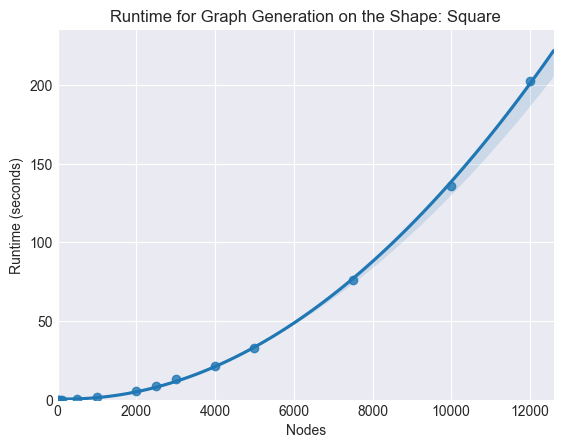
\includegraphics[width=0.5 \textwidth]{square/runtime/runtime_chart_naive}
    \caption{Data on the Runtime of the $O(n^2)$ Algorithm}
  \end{figure}

  \begin{figure}[!htb]
    \centering
    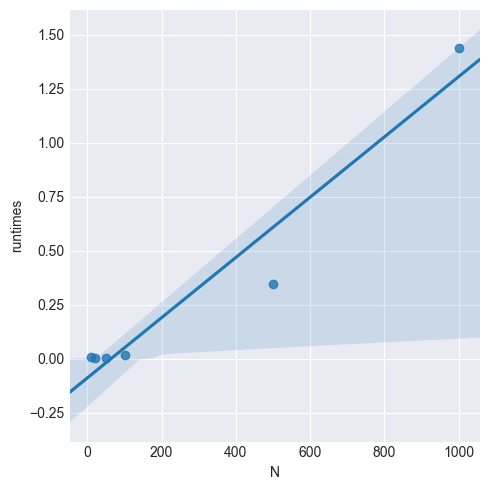
\includegraphics[width=0.5 \textwidth]{square/runtime/runtime_chart}
    \caption{Data on the Runtime of the $O(n)$ Algorithm}
  \end{figure}

\section{Result Summary}

\end{document}
